\chapter{永恒探索算法}

离散模型中,探索空间一般抽象为一个无向连通图,图的每个结点代表空间上机器人可达的位置,边代表机器人可以通过的路径,机器人沿着该路径到达相邻的空间位置。空间中每个位置结点在同一个时间至多只有一个机器人。

\begin{figure}[!hbt]
	\centering
	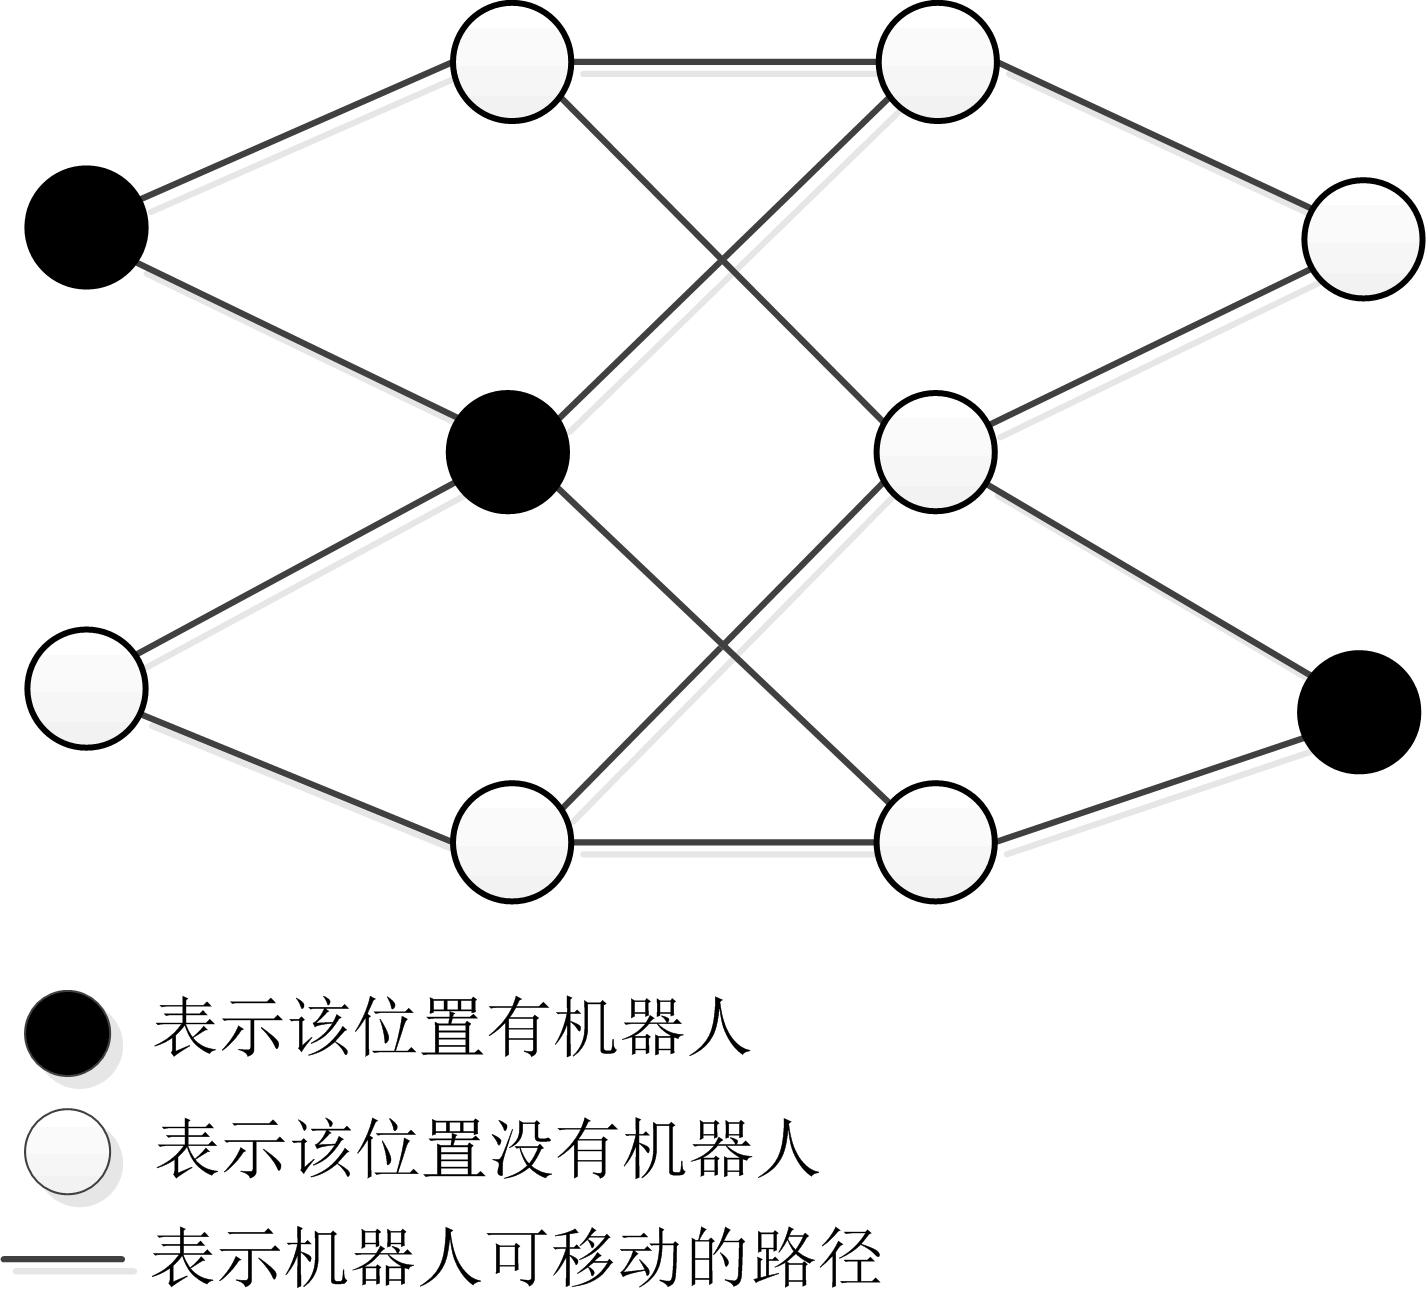
\includegraphics[width=3 in]{fig/normalspace.png}
	\caption{无向连通图表示探索空间}
	\label{fig:normalspace}
\end{figure}

如图\ref{fig:normalspace}给出了一个简单的离散探索空间的无向连通图表示,黑色结点表示该空间位置在此刻有一个机器人,白色结点说明该空间位置上没有机器人,图中有三个机器人,分别位于三个黑色的空间结点上。类似于计算机网络拓扑结构,探索空间结构也有总线拓扑结构、星型拓扑结构、环形拓扑结构、树形拓扑结构等。

\section{机器人移动三个阶段}
离散空间上每个机器人的移动分为三个阶段,分别是观察(look)、计算(compute)和移动(move).在观察阶段,机器人通过自身的视觉传感器,获取空间环境中其他机器人的位置快照信息。然后进入计算阶段,计算阶段根据观察阶段获取的位置快照信息,匹配自身预先设置的移动算法,计算得出下一步的移动策略。移动策略包括机器人是否移动,若是移动,则是沿着那条路径进行。移动阶段,机器人的动力装置按照计算阶段的所得移动决策作出对应的移动。

\begin{figure}[!hbt]
	\centering
	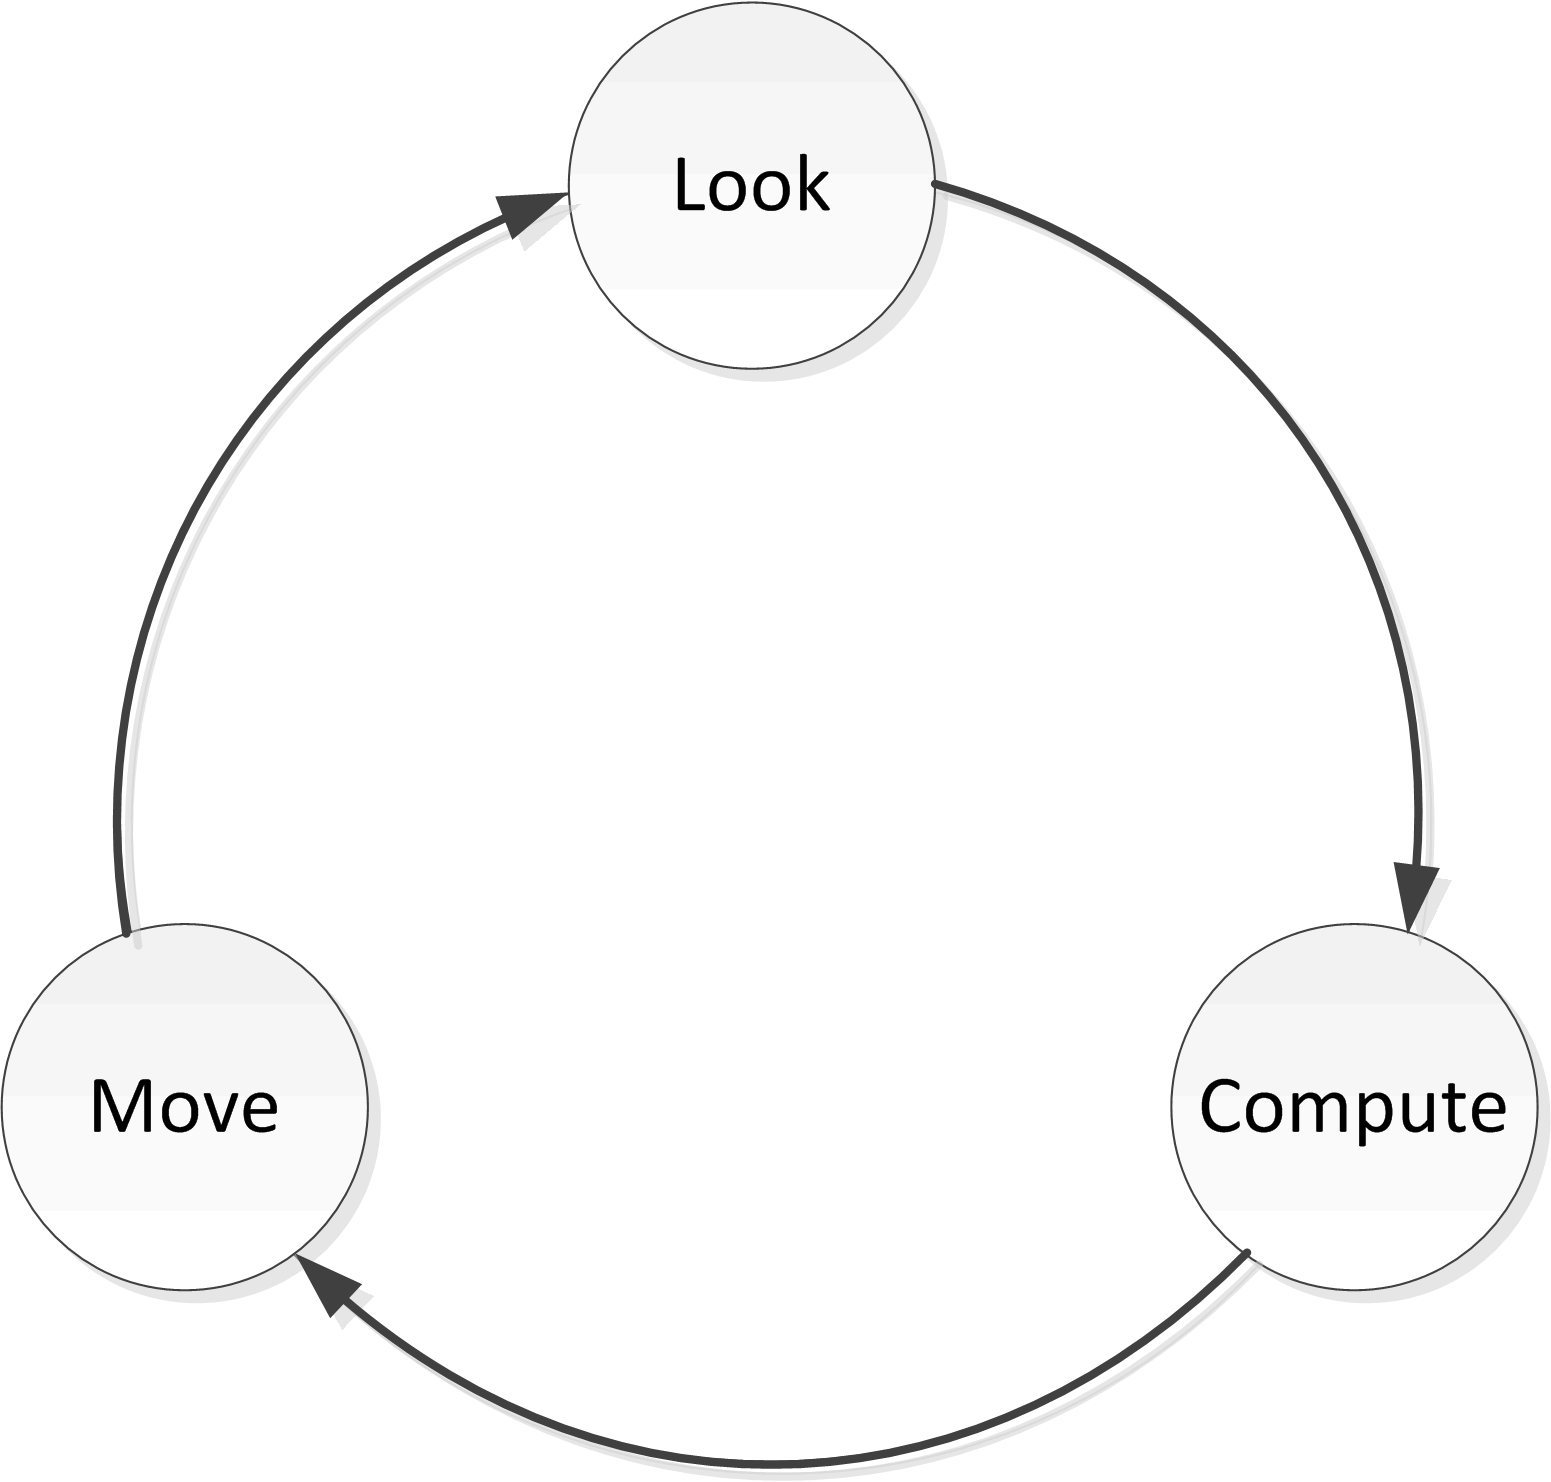
\includegraphics[width=3 in]{fig/robotthreephase.png}
	\caption{机器人移动三阶段}
	\label{fig:robotthreephase}
\end{figure}

如图\ref{fig:robotthreephase}描述了机器人移动的三个阶段,这三个阶段按照观察阶段、计算阶段、移动阶段,完成移动阶段之后又进入观察阶段,这样不断重复三个移动阶段。

\section{机器人移动调度策略}
原有模式中,Suzuki假设空间中机器人个数大于0,机器人的移动三个阶段具有原子性,且机器人之间的运动过程是同步的,提出了移动调度策略的两种变体,分别是完全同步调度模型FSYNC(fully-synchronous model)和半同步调度模型SSYNC(semi-synchronous model)。 后来由Flocchini等人提出了异步调度模型ASYNC (asynchronous model),该异步调度模型中,机器人观察,计算,移动三个移动阶段不再具备原子性,这样可能会出现机器人使用过时的快照信息做出移动决策。

下面使用数学和算法知识来描述完全同步调度模型、半同步调度模型、异步调度模型具体的内容。

假设在一个离散空间中存在$k\left(k \in N^+ \right)$个机器人,使用集合$Rob =\left\{r_1,r_2,r_3,...,r_k\right\}$ 表示。空间位置结点可以按照一定顺序,对其进行编号,编号是空间位置结点的唯一标识,使用集合$Pos =\left\{n \in N^+ |0,1,2,...,n-1\right\}$ 表示空间所有空间位置结点,每个元素对应唯一一个空间位置结点。机器人是在空间位置结点上的,所以机器人与空间位置结点的映射关系使用$p:\left\{Rob \rightarrow Pos\right\}$表示,机器人r 在某个时间所在图中的位置结点编号就为$p\left(r \in Pos \right)$。对于Rob 中的任意两个机器人$r_i,r_j\left(i \neq j \right)$, 在任意一个时刻满足位置结点不相同$p\left(r_i\right) \neq p\left(r_j\right)$, 即空间中任意时刻一个位子结点上至多只有一个机器人。

前面使用数学中的集合和映射定义了探索的离散空间、机器人已经机器人在空间结点上的函数关系,在此基础上,下面将介绍机器人移动的三种调度模型。完全同步调度模型是半同步调度模型的一种特殊情况,所以先介绍半同步调度模型,在介绍完全同步调度模型。完全异步调度模型完全与前面两种调度模型由较大区别,所以放在最后介绍。

将机器人移动的一个完整的观察、计算、移动称为完整移动阶段,在半同步调度模型中,Rob集合中只有选中的机器人才进行完整移动阶段。而半同步调度模型所有机器人都是同步而且观察、计算、移动都是具备原子性,所以可以每次选中的机器人是一个非空集合$Sched  \subseteq Rob $,在一个完整移动阶段开始之前,只有选入集合Sched的机器人才会执行完整移动阶段,即$\forall r \in Sched$执行观察、计算、移动,而$\forall r \notin Sched  $不执行。等到下一个完整移动阶段之前,又会从Rob 随机选择一个机器人$Sched  \subseteq Rob $,重复上述过程。这就是半同步调度模型机器人调度的性质。下面使用简易算法过程,详细描述一下半同步调度模型中机器人执行完整移动阶段的过程。

\begin{lstlisting}
SSYNC-SCHEDULE(Rob)
  while
    choose Sched from Rob
    synchronous {
       foreach r in Sched{
          r.look
          r.compute
          r.move
       }
    }
\end{lstlisting}

半同步调度模型SSYNC-SCHEDULE的传入参数是机器人集合Rob,首先从Rob集合中选择子集合Sched且$Sched \neq \emptyset$。关键字\verb|synchronous| 表示同步块中所有机器人同步完成移动阶段。在Sched 集合中的每个机器人开始同步执行观察、计算、移动。完成之后,又重新开始随机选择子集合Sched,重复不断执行上述过程。

完全同步调度模型是半同步调度模型中一种很特殊的情况,每次随机选择的集合$Sched = Rob $,即每次完整移动阶段之前在集合Rob 中所有的机器人都被选中。使用算法过程描述如下:

\begin{lstlisting}
FSYNC-SCHEDULE(Rob)
  while
    synchronous {
       foreach r in Sched{
          r.look
          r.compute
          r.move
       }
    }
\end{lstlisting}

同半同步调度模型相对较而言,完全同步调度模型只是在每次选择集合$Sched$有所不同,其他过成完全相同。

而完全异步调度模型中,所有的机器人观察、计算、移动都是异步,没有原子性。类似于计算机系统的多线程,每个机器人的移动都是并行且互相之间没有同步约束,当一个机器人在观察时,其他机器人可能在执行计算或者移动。每个机器人执行移动的快慢完全是随机的,所以肯能会出现机器人在观察阶段通过视觉传感器获得快照是过时的。

\begin{lstlisting}
ASYNC-SCHEDULE(Rob)
    asynchronous {
       foreach r in Rob{
           while{
              r.look
              r.compute
              r.move
           }
       }
    }
\end{lstlisting}

上述完全异步调度模型算法中,关键字\verb|synchronous|表示Rob中所有的机器人都异步执行移动,对于每个机器人而言,都是在按照顺序不断重复执行观察、计算和移动过程,即整个过程中机器人都是并行执行完整移动阶段。

\section{环形空间探索算法}
探索空间结构有总线拓扑结构、星型拓扑结构、环形拓扑结构、树形拓扑结构,不同的探索空间结构有各自的特点,本文以环形拓扑结构空间为例.首先介绍环形拓扑结构环上的机器人视觉快照、匹配移动算法获取移动决策、移动决策的执行.在此基础上,将介绍永恒探索移动算法的相关概念.

\subsection{机器人视觉快照}
图\ref{fig:ring}给出一个简单的环形拓扑结构探索空间的例子。根据环形空间的自身特点,沿着环的顺时针方向,从\verb|0| 开始递增进行编号。所有位置编号组成的集合为Pos,图中黑色结点表示该位置结点上有机器人,白色结点表示该位置结点上没有机器人。下面给出某个时刻某个结点上机器人的数量的定义。

\vspace{0.5cm}

\begin{figure}[!hbt]
	\centering
	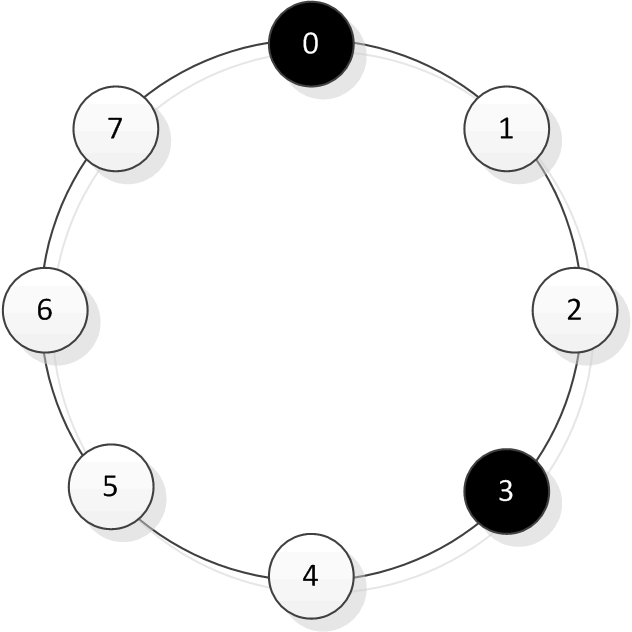
\includegraphics[width=2 in]{fig/ring.png}
	\caption{环形拓扑结构探索空间}
	\label{fig:ring}
\end{figure}

\vspace{0.5cm}

\begin{bfseries} 定义1\quad(机器人所在位置编号)\end{bfseries}对于机器人\verb|r|,其所在探索空间中位置的编号使用符号$c_{\left(r\right)}$,$c_{\left(r\right)} \in Pos$。

\vspace{0.5cm}

\begin{bfseries} 定义2\quad(结点机器人个数)\end{bfseries}结点机器人数$d_j$,\verb|j|表示结点的编号$j \in Pos $,当结点\verb|j|上有$k \left(k > 0\right)$机器人表示为$d_j = k$, 本文中同一时刻每个结点至多有一个机器人,在结点上存在机器人时$d_j = 1$, 当结点\verb|j| 没有机器人时,表示为$d_j = 0$。

\vspace{0.5cm}

在环形拓扑结构的离散空间中,空间中的每个机器人可以顺时针观察,也可以逆时针观察。那么机器人每次观察的位置信息快照就有顺时针位置信息快照和逆时针位置信息快照两种,为了方便描述,给出某个位置上机器人获取位置信息快照的定义,如下:

\vspace{0.5cm}

\begin{bfseries} 定义3\quad(机器人快照)\end{bfseries}离散空间上位置结点$p \in Pos$,\verb|j|上的机器人通过视觉传感器获取的位置快照为$\delta_p^F$,其中$F \in \left\{+,-\right\} $,\verb|+|表示顺时针,\verb|-|表示逆时针。

\vspace{0.5cm}

在拥有\verb|n|个位置结点的环形拓扑结构的探索空间上,任意位置结点\verb|j|上机器人的顺时针和逆时针快照如下:

\verb|顺时针序列定义:| $\delta_p^+ = \left\langle d_j,d_{j+1},...,d_{j+n-1}  \right\rangle.$

\verb|逆时针序列定义:| $\delta_p^- = \left\langle d_j,d_{j-1},...,d_{j-n+1}  \right\rangle.$

如图\ref{fig:ring}中以位置编号为0的结点为例,其结点上机器人的顺时针和逆时针位置信息快照如下:

\verb|顺时针序列1:| $\delta_0^+ = \left\langle 1,0,0,1,0,0,0,0  \right\rangle.$

\verb|逆时针序列1:| $\delta_0^- = \left\langle 1,0,0,0,0,1,0,0  \right\rangle.$

虽然上述位置快照信息描述比较简洁和直观,但是当空间结点数n较大时,位置快照信息就过长,不利于描述。后来由lelia.blin在其文献[Ring]中提出了一种新的位置快照\verb|F-R|表达方式,\verb|F-R|表达方式中使用$F_m$ 表示连续的\verb|m|个空间位置结点上没有机器人,$R_n$表示连续的\verb|n|个空间位置结点上有机器人。那么顺时针序列1 和逆时针序列1转化为F-R的表达方式为:

\verb|顺时针F-R序列1:| $\delta_0^+ = \left\langle R_1,F_2,R_1,F_4  \right\rangle.$

\verb|逆时针F-R序列1:| $\delta_0^- = \left\langle R_1,F_4,R_1,F_2   \right\rangle.$

\vspace{0.5cm}

\begin{bfseries} 定义4\quad(机器人快照F-R表达式)\end{bfseries}\verb|k|$\left(k \in N^+  \right)$个机器人在\verb|n| $\left(n \in N^+  \right)$个位置结点环形空间中,且$k < n$,使用符号\verb|R|和\verb|F|所组成的符号序列表示机器人快照。带下标的$R_i$表示连续\verb|i|个空间位置结点,每个位置结点被一个机器人占据。带下标的$F_j$表示连续\verb|j|个空间位置结点,每个位置结点上都没有机器人。

\vspace{0.5cm}

机器人快照\verb|F-R|表达式不仅可以解决环形空间结点数n较大,不易描述的问题,而且可以通过下角标使用未知变量,表达连续没有机器人位置结点数和有机器人位置结点数,增强了表达式的灵活性、可读性和表达能力。

\subsection{机器人移动算法}
机器人移动算法是保证自主机器人协同完成设的任务的核心,在同一个探索空间中的机器人都预先设置完全相同的移动算法。机器人的可能的移动策略取决于其所在探索图形状,本小节主要介绍环形探索图中的机器人移动算法。

环形探索图中,对于某个位置结点\verb|g|上的机器人来说,若其视觉快照$\delta_g^+ = \delta_g^-$,称为对称(symmetry)。由于对称情况的存在,所以机器人的移动存在四种方式:不移动$\left(Idle\right)$、 前进$\left(Front\right)$、后退$\left(Back\right)$、 未确定$\left(Doubt\right)$。未确定的情况是位置结点上的机器人顺时针视觉快照和逆时针视觉快照相同,那么该结点上机器人可能前进或者后退。未确定表示此时机器人随机选择前进或者后退。

本文中的机器人移动算法,是机器人快照F-R表达式和对应四种移动方式组合而成。下面使用机器人最小移动算法为例,详细介绍机器人移动算法。最移动算法是指环形探索空间中,空间位置结点数$n \geq 10$,图上的机器人$k = 3$,且\verb|n|和\verb|k|数量关系上互质。最移动算法分为两个阶段:稳定阶段$\left(Legitimate\quad phase\right)$和收敛阶段$\left(Convergence\quad phase\right)$。

\vspace{0.5cm}

\begin{table}[hbt]
    \centering
    \caption{最小移动算法稳定阶段}
    \begin{tabular}{|p{2cm}|p{8cm}|p{2cm}|p{2cm}|}
        \hline
        $RL1$&$\delta_{c\left(r\right)}^F = \left\langle R_2,F_2,R_1,F_{n-5} \right\rangle.$&$\rightarrow$&$r.Back$\\
        \hline
        $RL2$&$\delta_{c\left(r\right)}^F = \left\langle R_1,F_1,R_1,F_{n-6},R_1,F_2 \right\rangle.$&$\rightarrow$&$r.Front$\\
        \hline
        $RL3$&$\delta_{c\left(r\right)}^F = \left\langle R_1,F_3,R_2,F_{n-6}\right\rangle.$&$\rightarrow$&$r.Front$\\
        \hline
    \end{tabular}
    \label{table:minalgotithm}
\end{table}

\vspace{0.5cm}

\begin{figure}[!hbt]
	\centering
	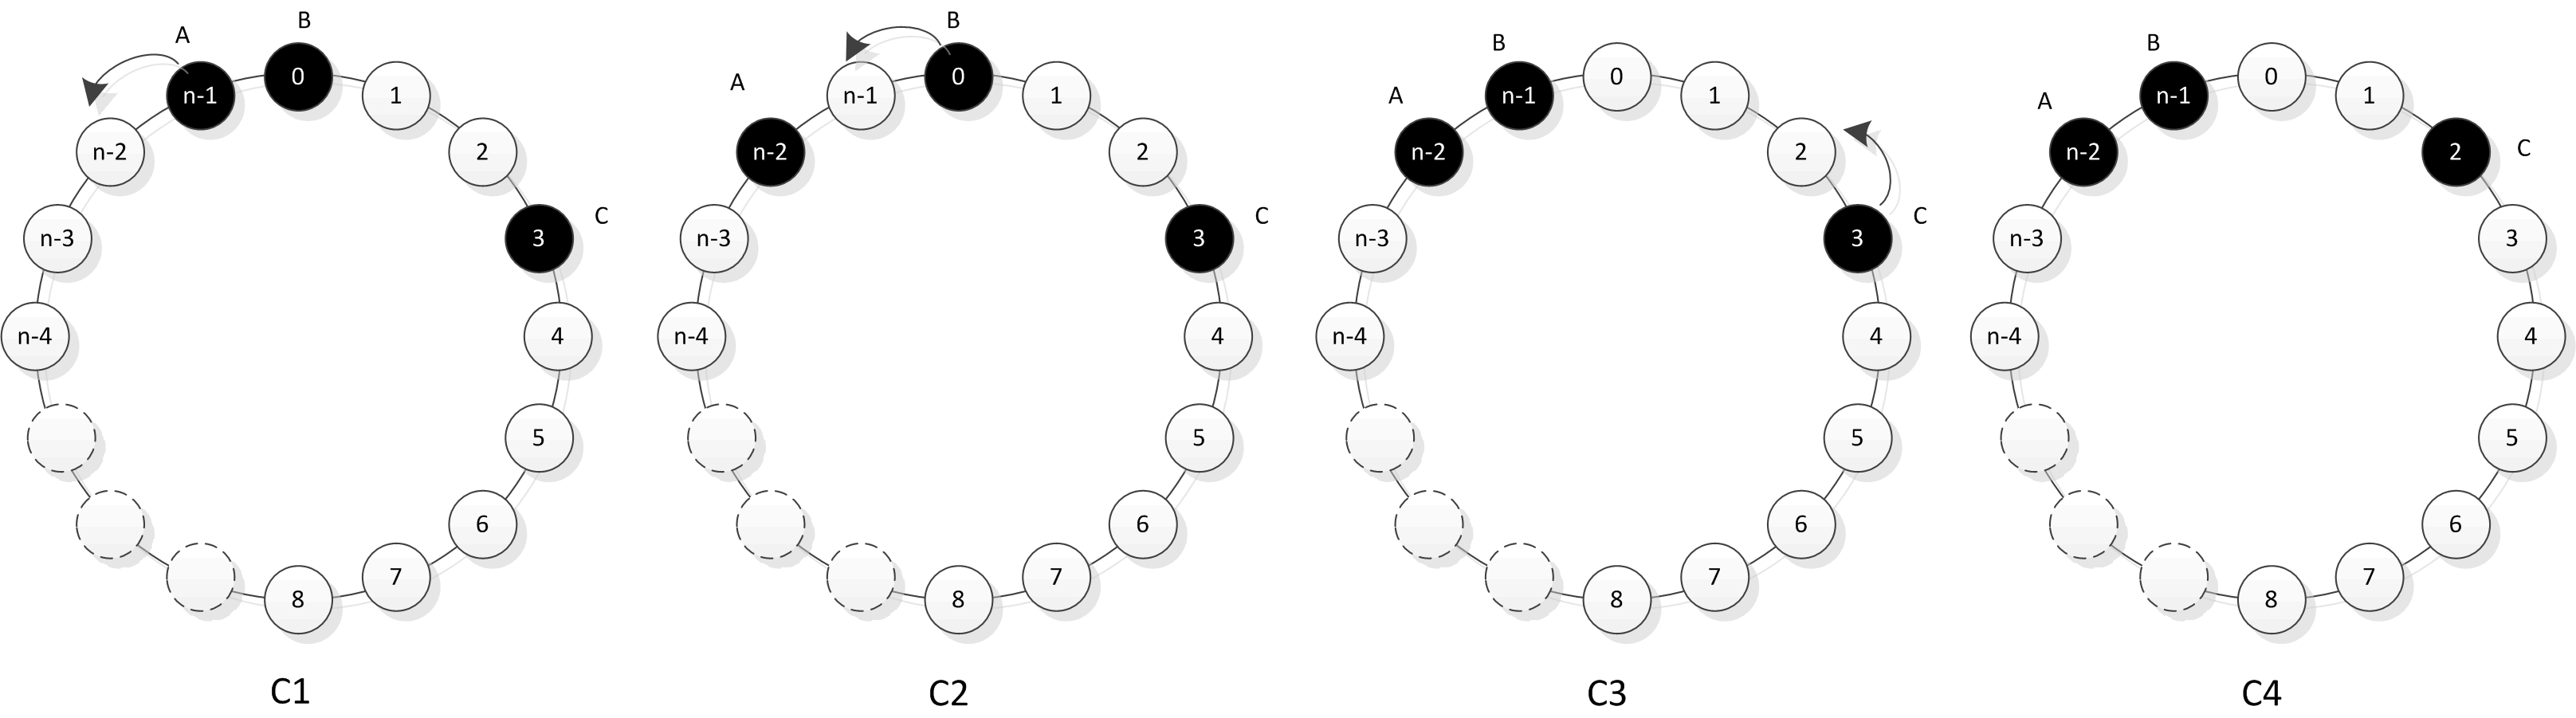
\includegraphics[width=6.5 in]{fig/perpetualexploration.png}
	\caption{最小移动算法的稳定阶段}
	\label{fig:perpetualexploration}
\end{figure}

\vspace{0.5cm}

在图\ref{fig:perpetualexploration}中,给出了三个机器人按照预设的稳定阶段算法运动过程的例子,C1 中机器人A 的顺时针位置信息快照${delta_{c\left( A\right)}^+}$匹配移动算法$RL1$做出后退的移动决策,机器人A从位置结点$n-1$移动到$n-2$,其他机器人$B$和$C$此时没有匹配任何移动算法,保持静止。C2 中机器人B 的逆时针位置快照${delta_{c\left( B\right)}^-}$匹配移动算法$RL2$,做出前进的移动决策,机器人A从位置结点$0$移动到$n-1$。 同样机器人C 的逆时针位置快照信息,匹配移动$RL3$做出前进的移动决策。图中C1和C4进行对比,图中三个机器人的位置都向顺时针移动了一位,C4中A获取的位置信息F-R 表达式同C1 中的A 获取的位置信息F-R表达式相同。意味着整个系统会按照上述C1到C4过程重复执行,而且每次执行之后,所有机器人都会向逆时针方向移动一位。这说明系统进入了稳定阶段,稳定阶段的系统状态称为稳定状态。系统进入稳定状态之后,就会一直停留在稳定阶段中。介绍了最小移动算法的稳定阶段之后,下面介绍其收敛阶段。

\begin{table}[hbt]
    \centering
    \caption{最小移动算法收敛阶段}
    \begin{tabular}{|p{2cm}|p{8cm}|p{1cm}|p{2cm}|}
        \hline
        $RC1$&$4 \leq x \leq z  \land \delta_{c\left(r\right)}^F = \left\langle R_1,F_x,R_2,F_z\right\rangle.$&$\rightarrow$&$r.Front$\\
        \hline
        $RC2$&$x \neq y,x>0 \land \delta_{c\left(r\right)}^F = \left\langle R_1,F_x,R_1,F_y,R_1,F_x\right\rangle.$&$\rightarrow$&$r.Doubt$\\
        \hline
        $RC3$&$0<x<z<y \land \left( x,y \right) \neq  \left( 1,2 \right)\land \delta_{c \left(r\right)}^F = \left\langle R_1,F_3,R_2,F_{n-6}\right\rangle.$&$\rightarrow$&$r.Front$\\
        \hline
        $RC4$&$\delta_{c\left(r\right)}^F = \left\langle R_3,F_{n-3}\right\rangle.$&$\rightarrow$&$r.Back$\\
        \hline
        $RC5$&$\delta_{c\left(r\right)}^F = \left\langle R_1,F_1,R_2,F_{n-4}\right\rangle.$&$\rightarrow$&$r.Back$\\
        \hline
    \end{tabular}
    \label{table:minalgotithmconvergence}
\end{table}

在表\ref{fig:minalgotithmconvergence}中,是最小算法的收敛算法,系统状态除了稳定状态之外的都称为收敛状态,系统任意收敛状态都可以通过收敛算法到达稳定状态。下面将以最小移动算法为例,具体介绍系统如何从任意的一个状态到达稳定状态。

\vspace{0.5cm}

\begin{figure}[!hbt]
	\centering
	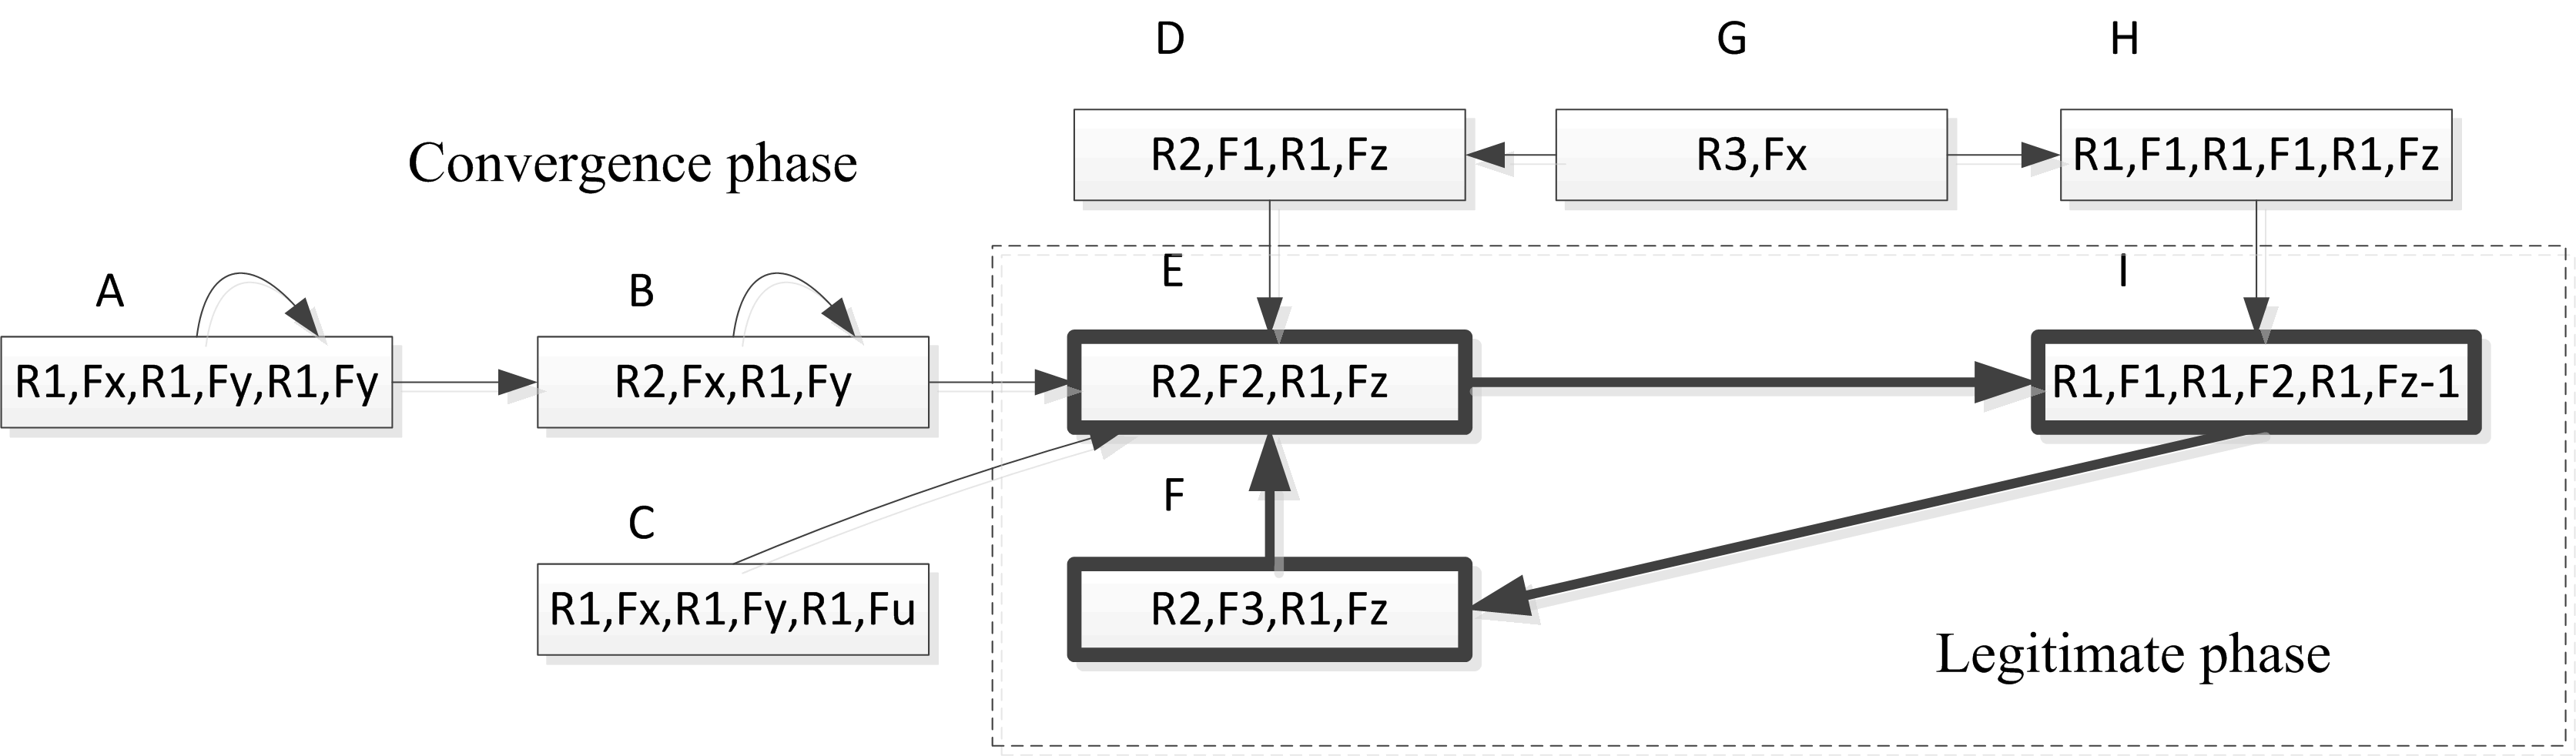
\includegraphics[width=6 in]{fig/cp_lp.png}
	\caption{最小机器人移动算法状态转移}
	\label{fig:cp_lp}
\end{figure}

\vspace{0.5cm}

图\ref{fig:cp_lp},描绘了完全同步调度模型和半同步调度模型中,最小移动算法中的稳定阶段和收敛阶段的所有状态,移动机器人所在空间位置结点上的视觉快照,匹配移动算法中状态,满足则按照对应的移动策略做出移动动作。每当机器人做出移动之后,空间中位置信息就会发生变化,系统的状态发生改变。虚线方框中的表示稳定阶段的三种状态,构成了有向强连通图。进入稳定阶段的状态,就会在三种状态之间按照箭头指向顺序,不断重复转换,再也不能进入除此三种状态以外的状态了。对于虚线以外的状态称为收敛状态,收敛状态可以通过收敛算法逐渐到达稳定状态。

\section{探索终止和永恒探索}
由Flocchini在文献[1]提出了探索终止(exploration with stop)问题,所谓探索终止是指空间中每个位置结点都会被至少一个机器人访问一次,在空间上每个结点都被访问之后,所有机器人都停止不动。Flocchini证明了环形空间,位置结点数n 和机器人数k ,若n对k取模为0,那么没有移动算法满足探索终止性质。同时,文献中给出一组确定性的移动算法,在机器人数$k \geq 17$,机器人数k与结点n互质时,满足探索终止性。永恒探索(perpetual exclusive exploration) 是指空间中每个机器人对空间中的每个结点重复的访问,并且该过程是不停止的。

探索终止和永恒探索是都是自主机器人对空间位置结点的巡查模式,这两种巡查模式都是确保机器人协作完成预设探索空间任务的方式。探索终止和永恒探索只有微小区别,在本质上是所有空间位置结点都被机器人访问。本小节介绍探索终止和永恒探索具体内容。

\subsection{探索终止}
对于环形探索空间来讲,无论空间中所有机器人在什么初始位置,给出一个移动算法使得机器人组在有限时间内满足探索终止。这可以归纳为两条性质,如下:

\vspace{0.2cm}

\begin{bfseries}探索性(Exploration):\end{bfseries}环上每个结点至少被一个机器人访问。

\begin{bfseries}终止性(Termination):\end{bfseries}在满足探索性前提下,最终到达某一状态使得所有的机器人都保持静止,不再移动!

\vspace{0.2cm}

对于第二条性质而言,要求机器人"记住"环形探索图中有多少位置结点已经被访问了,即这些没有记忆存储的机器人通过它们当前获取的视觉快照,区分探索过程中不同阶段。这两种属性也可以使用LTL公式来表示,如下:

\vspace{0.2cm}

\begin{bfseries}探索性(Exploration):\end{bfseries}$\bigwedge_{j=0}^{n-1} \Diamond \left(d_j>0\right) $。

\begin{bfseries}终止性(Termination):\end{bfseries}$\bigwedge_{j=0}^{n-1} \Diamond \left(d_j>0\right)  $。

\vspace{0.2cm}

\subsection{永恒探索}
对于一个环形探索空间中,机器人任意初始状态,每个机器人在预设的移动算法下,都可以对环形探索空间中的任意一个位置结点无限反复的进行访问。对于同于的位置结点而言,在同一时刻至多只能有一个机器人占据,称为非冲撞性(No collision)。对于相邻的两个机器人,不能同时通过相邻边互换空间位置,即相邻的两个机器人不能在相邻的边上发生碰撞,该性质称为非互换性(No switch)。 环形图中每个机器人都必须对探索空间中任何一个位置结点进行反复的访问,且永不停止,称为非终止性(Live)。上述三条性质就是永恒探索内在意义,满足上述三条性质的算法称为永恒探索算法。下面使用LTL公式分别描述这三条性质:

\vspace{0.2cm}

\begin{bfseries}非冲撞性(No collision):\end{bfseries}$\bigwedge_{i=1}^{k} \bigwedge_{j=1}^{k} \Box \left(i \neq j \rightarrow c_{r_i} \neq c_{r_j}\right) $。

\begin{bfseries}非互换性(No switch):\end{bfseries}$\bigwedge_{h=0}^{n-1}\bigwedge_{i=1}^{k}\bigwedge_{j=1}^{k}  \Box \left(c\left(r_i\right)=h \land  c \left(r_j \right) = \left(h + 1 \right) mod \ n $
$ \rightarrow \Chi \left( \urcorner  \left(c\left(r_i\right)  = \left(h+1\right) mod \ n    \right)   \land c\left(r_j\right) =h \right)   \right)$。

\begin{bfseries}非终止性(Live):\end{bfseries}$\bigwedge_{h=0}^{n-1} \bigwedge_{i=1}^{k} \Box \Diamond \left(c\left(r_i\right)=h\right)$。

\vspace{0.2cm}

上述三条LTL公式描述性质中,n表示探索空间的位置结点数,k表示探索空间中的机器人数。在异步调度模型中,上述三条性质都必须在公平性为前提,即任何一个机器人都可以被无限次的调度,才能满足永恒探索。公平性的LTL 公式描述如下:

\vspace{0.2cm}

\begin{bfseries}公平性(Fairness):\end{bfseries}$\bigwedge_{i=1}^{k} \Box \Diamond \left(r_i.running = true\right)$。

\vspace{0.2cm}

\section{本章小结}
本章首先使用数学定义方式,分别描述了空间位置结点,机器人移动的三个阶段观察、计算和移动。将机器人移动的三个阶段是否有原子性,以及机器人是否同步移动为调度模型的划分依据,介绍了三种调度模型完全同步调度模型、半同步调度模型和异步调度模型。介绍了机器人视觉快照表达式,F-R视觉快照表达式更加灵活,且表达能力更强。移动机器人算法是以视觉快照为依据,所以移动机器人算法是以视觉快照和对应的预设移动组合的式子,后续由以最小移动算法为例,讲解了稳定阶段和收敛阶段。自主移动机器人的核心是机器人协作完成预设任务,所以介绍了探索终止和永恒探索两种任务问题,并使用LTL公式具体描述了其满足的性质。